\chapter{APRS RF Channel Capacity}
\label{chap:channelcapacity}

One of the largest limitations of the APRS network is the fact that it primarily operates
on a single regional 1200 bits per second data channel. 
Individual nodes share the 1200bps channel using 
CSMA as discussed in section~\ref{sec:bell202csma}, but the relationship between 
these channel access methods and how often a station should beacon isn't straight-forward.

The APRS specification fails to give concrete guidance on what beacon interval should
be used beyond stating that every station should beacon at the net's cycle rate,
which it lists as 10 minutes locally and 30 minutes 
network wide\cite[p.~9]{aprsspec}.\footnote{see proportional pathing in the previous section}
For fixed nodes such as weather stations and network infrastructure, 
these intervals are appropriate, but mobile users find this beacon interval unsatisfying
and not useful.
There is a common desire to beacon more often than every 10 minutes,
as shown by the wide deployment of SmartBeaconing,
but how often is allowable while staying within the limitations of the network?

This chapter will give an introduction to the original ALOHAnet research that networks like
APRS are based on, and point out how these models fall short of the actual APRS network,
but a comprehensive study of the specifics as applied to APRS are beyond
the scope and resources of this work.

\section{Network Capacity Objectives}

The stated objective of APRS is to pass real-time tactical information among a station's
60 closest peers.
This value was apparently selected arbitrarily based on the feeling that
it is unlikely that a station would need to interact with anyone beyond their 60
closest peers, but will nevertheless be used for the analysis in this chapter.
This does complicate analysis of the APRS network since each station's set of
their 60 nearest peers, which is referred to as their ``Aloha Circle,"
is a different subset of all the stations in the network;
every station has a different point of view as to who is in their aloha circle and who
is not.
Analysis is further complicated by the fact that few APRS stations are actually within
radio range of 60 other stations, so often a significant portion of an aloha circle is
beyond the local horizon and relayed through digipeaters.
This effects a phenomenon call the ``hidden node problem," which impacts
layer 1 CSMA access, which for the sake of simplicity is ignored in this introduction.

An appropriate starting point for analyzing APRS channel capacity would be the original methods
developed for the ALOHA System at the University of Hawaii\cite{packetthroughput}.
The ALOHAnet was a 9600bps UHF packet radio system that was the first application of 
wireless computer networking.
This system developed several of the shared channel access methods 
that would subsequently be used in other protocols such as Ethernet, GSM, and APRS.

\section{Poisson Channel}

The most basic analysis of a channel's ALOHA capacity can be based on the assumption that
each packet is the same length, 
that traffic enters the network as a Poisson process,
and that any collision between two packets causes both of them to fail to be delivered.
Defining the rate of packets entering the network as $\lambda$ in packets per second and
the length of each packet as $\tau$ in seconds, the normalized channel traffic G can be
calculated as
\begin{equation}
	G = \lambda \tau
\end{equation}
This normalized value is measured in units of Erlangs,
which indicate what fraction of a channel would be needed for all
of the traffic entering the network.
For example, a value $G=1.0$ would indicate that
a single station would need to transmit packets continuously, where $G=0.5$ indicates 
a free channel half the time.
Erlang values above one are valid, and simply represent that multiple separate
channels would be needed to handle all of the traffic.

Unfortunately, when channel access is stochastic,
there is no guarantee that two stations won't transmit at the same time.
Any packet transmission starting less than $\tau$ seconds before or after another would
cause a collision and both packets would be lost.
This indicates that the rate of successfully received packets exiting the network may
be lower than $\lambda$, and is traditionally notated as $\lambda'$. 
Since $\lambda' \leq \lambda$, we define the normalized channel throughput S as
\begin{equation}
	S = \lambda' \tau
\end{equation}
Due to the assumption that the channel access is Poisson, 
the probability that a packet will collide with another is $e^{-2 \lambda \tau}$,
which therefore yields the relationship between S and G of
\begin{equation}
	S = G e ^ {-2 G}
\end{equation}
This indicates a moderately surprising result that for Poisson channel access,
the throughput is completely independent of the number of stations on the channel,
but only dependent upon the total channel loading.

\begin{figure}
	\centering
	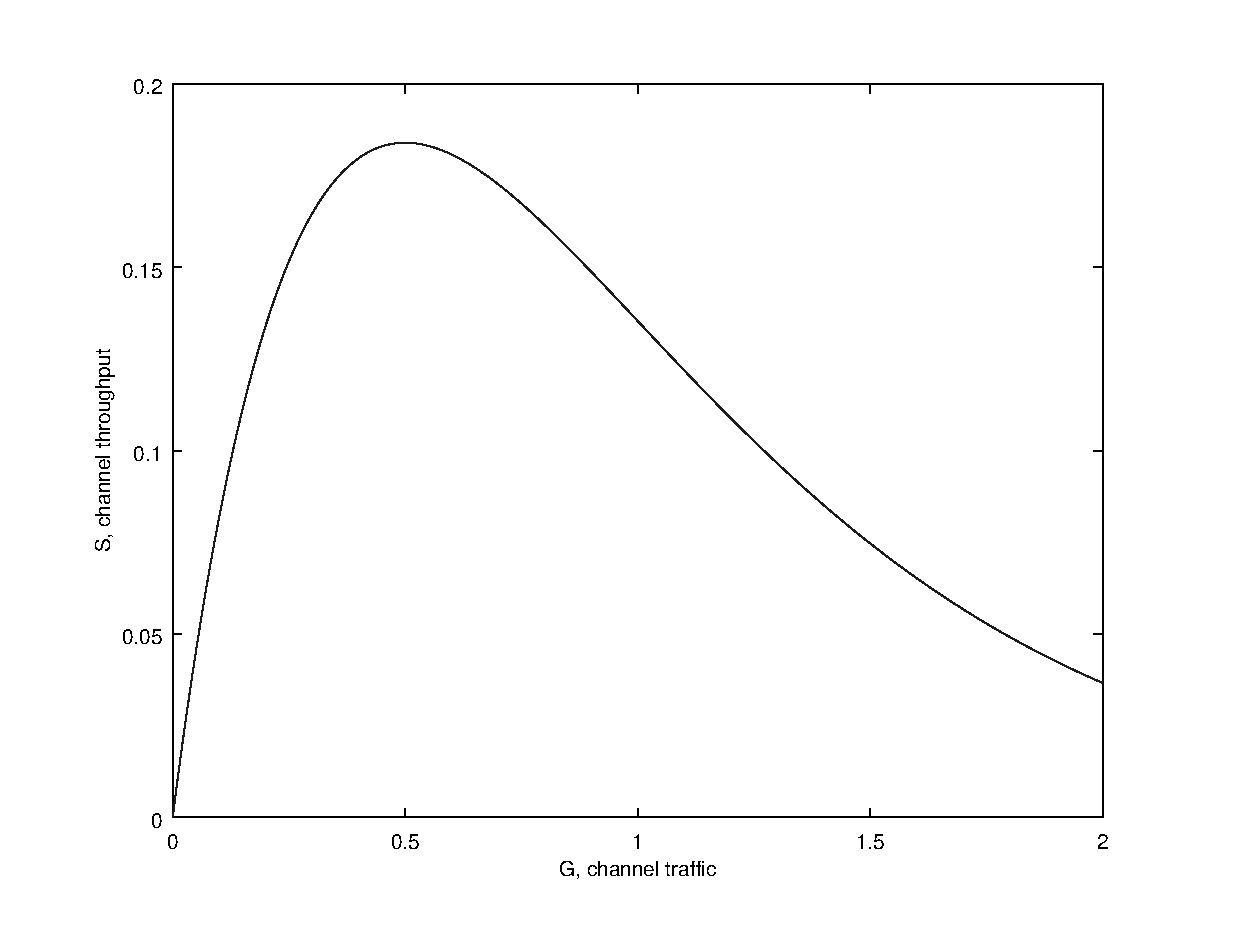
\includegraphics[width=1.0\textwidth]{src/octave/poissonthroughput}
	\caption{Poisson channel traffic and throughput}
	\label{fig:SGpoisson}
\end{figure}
Graphing the channel throughput versus the channel's traffic yields figure 
\ref{fig:SGpoisson}, which indicates that as you increase channel traffic, 
throughput increases to an inflection point when there is no unused channel capacity
and packet collisions finally start to dominate
the channel and harm throughput. This inflection point happens to be at
an incoming traffic $G = 0.5$ which yields an expectation that 36\% of the packets
will be successfully received ($S = 0.18$).

While assuming that APRS traffic is based on a Poisson process is 
highly suspect, this simple model of channel capacity does yield some insightful 
values. 
Collecting several days of APRS traffic on 144.390MHz in San Luis Obispo, California
shows an average packet size of 119 octets. With a typical 300ms preamble,
the assumption that every packet is the mean length,
and a data rate of 1200bps, this yields $\tau = 1.09$ seconds.
\begin{equation}
	\lambda_{APRS} = \frac{G_{MAX}}{\tau} = 0.457
	\label{equ:aprsmaxrate}
\end{equation}

Equation \ref{equ:aprsmaxrate} indicates that a single APRS channel can support
0.457 transmitted packets per second, or
27 packets per minute, which need to be shared between
all of the participating network nodes.
Assuming the typical target LAN size of 60 stations, 
this implies an average packet interval per station
of \emph{2 minutes 13 seconds}.\footnote{For the reader skimming this chapter, DO NOT
	use this beacon interval for APRS; this Poisson model is too simplified to give
meaningful results. A suggested default is 600 second intervals when beaconing.}
The less satisfying result is the fact that only 10 of these packets every minute will be
successful received, which indicates that
two thirds of the transmitted power is wasted.

The next section will go into how this Poisson model is deficient to the
point that this 2 minute 13 seconds value is nearly meaningless.
Any station that beaconed that fast on an actual APRS network could very quickly
be identified as abusive to the rest of the network, so further work is needed
before an analytic interval suggestion can be made.
What this calculation does demonstrate is that the general concept of 60 stations
sharing a single ALOHA channel in the way APRS intends is within the realm of
possibilities. 
Had this value come out an order of magnitude larger, the claim
that APRS could allow a user to discover 60 other stations would be much more suspect.

\section{Deficiencies of the Poisson Model}

There were several assumptions made to simplify the just-presented model 
for an ALOHA channel that are not particularly valid 
when applied to a typical APRS network. 
While most of these assumptions indicate that the result of
equation \ref{equ:aprsmaxrate} is overly optimistic and 
stations should beacon less often, there are enough different mechanisms at play
in both directions that the true traffic versus throughput relationship 
is not easily found and requires further work beyond this paper.
Some of the ignored issues include:

\begin{itemize}
	\item Differences in packet length -- Actual APRS traffic varies in length,
		which has an effect on throughput rates by changing $\tau$.
		Abramson considered the general
		case for two discrete packet lengths \cite{packetthroughput},
		but in general this encourages users to make packets as short as possible
		to improve throughput.
	\item Digipeaters and channel access methods -- The presented model assumes that
		every packet is added to the channel as an entirely blind shot in the dark,
		but many APRS stations use CSMA to avoid transmitting on already busy channels.
		This reduces the window for destructive collisions and thus reduces the ratio
		between the channel traffic G and the usable throughput S.
	\item Sources of entropy in the network -- Starting with a Poisson stochastic model
		implies a strong assumption that every packet starts at a random time independent
		of every other packet. Many APRS stations beacon on a fixed interval,
		such as 600 seconds, which makes that station's traffic very self-similar.
		Digipeaters also strongly break this assumption by their action of immediately
		repeating packets after they're originally transmitted.
		These digipeater echos aren't random at all.
		Papers have been written on the misuse of Poisson traffic models with regards
		to TCP/IP networks \cite{failureofpoisson}, and those arguments often apply
		equally well to the APRS network.
	\item The heterogeneous nature of APRS equipment -- Any closed-form analysis
		of APRS depends on each network node behaving in one of a small set 
		of possible behaviors. The home-brewed and come-as-you-are nature of APRS
		makes the cumulative behavior of the network at large much harder to model.
		Useful models would need to depend on careful measurement of the behavior of
		existing nodes, and likely use Monte Carlo methods to make meaningful
		statements about the system at large.
\end{itemize}

In the end, building a meaningful model for APRS network traffic will likely prove
to be surprisingly challenging.
Much of this derives from the unusual amount of latitude given to APRS implementations
by the lack of detailed specifications that causes the aggregate network to behave so
unpredictably.
For further work modeling APRS to deliver meaningful results,
it's likely that it will need to begin by making a decision on which existing nodes in the
APRS network are ``misbehaving" by some developed metric and exclude them from
any further analysis.

The community has been extremely reluctant to outright classify APRS hardware
as misbehaving in the past,
due to the embedded nature of APRS nodes that usually precludes any major
modifications in behavior of existing nodes.
Classifying a node as misbehaving often meant that the operator would need to
spend a significant amount of time and money outright replacing the deficient hardware.
As more APRS nodes move to open-source and/or reprogrammable implementations,
it's conceivable that updates to APRS behavior as resulting 
from future research may become merely difficult,
instead of utterly impossible.\footnote{For example, the open source aprx package is
	one of the most popular pieces of i-gate software on the network \cite{aprxpopular},
	and modern trackers like those from Argent Data often
enjoy firmware updates which are relatively easy to install.}

